\documentclass[conference]{IEEEtran}
% \usepackage{cite}
% \usepackage{amsmath,amssymb,amsfonts}
% \usepackage{algorithmic}
\usepackage{graphicx}
\usepackage{multirow}
\usepackage{booktabs}
% \usepackage{textcomp}
% \usepackage{xcolor}
\graphicspath{{./images/}}
\def\BibTeX{{\rm B\kern-.05em{\sc i\kern-.025em b}\kern-.08em
    T\kern-.1667em\lower.7ex\hbox{E}\kern-.125emX}}
\begin{document}

\title{Shallow Convolutional Neural Network Architectures for Music Genre Classification}

\author{\IEEEauthorblockN{George Herbert}
\IEEEauthorblockA{\textit{Department of Computer Science} \\
\textit{University of Bristol}\\
Bristol, United Kingdom \\
cj19328@bristol.ac.uk}
}

\maketitle

\begin{abstract}
In this paper I investigate the shallow convolutional neural network architecture proposed by Schindler et al. \cite{SchindlerLidyRauber} for the task of music genre categorisation.
In the first part of this paper, I attempt to replicate the results achieved by Schindler et al., while in the latter part, I extend on their work by 
\end{abstract}

\begin{IEEEkeywords}
music information retrieval, convolutional neural networks
\end{IEEEkeywords}

\section{Introduction}

Music genre classification---categorising a music sample into one or more genres---is a fundamental problem in music information retrieval.
Early approaches to genre classification, such as that by Tzanetakis and Cook \cite{TzanetakisCook}, focused on training statistical classifiers using features such as timbral texture, rhythmic content and pitch content.
More recently, convolutional neural networks (CNNs) have been widely investigated in the context of genre classification, following their successes in the field of computer vision.

In one such paper, Schindler et al. \cite{SchindlerLidyRauber} investigated the performance of two different CNN architectures; in conjunction, they examined how data augmentation applied to four different datasets impacted the performance of both architectures.

\section{Related Work}

\section{Dataset}

I used the the GTZAN dataset compiled by Tzanetakis and Cook \cite{TzanetakisCook} to train and validate my models; it contains 1000 WAV audio tracks, each 30 seconds in length.
There are 100 tracks for each of the 10 genres in the dataset: blues, classical, country, disco, hip-hop, jazz, metal, pop, reggae and rock.
The CNNs were trained on chunks of approximately 0.93 seconds that were randomly selected from each audio track.

To produce a training and test set, a stratified split was deemed suitable to prevent imbalance.
Chunks from 75\% of the WAV audio tracks for each genre were randomly selected to make up the training set, with chunks from the other 25\% of audio tracks for each genre making up the test set.

\section{CNN Architecture (Schindler et al.)}

I recreated the shallow CNN architecture outlined by Schindler et al.
Log-mel spectrograms of shape $80\times80$ are provided as input to the network.

Since the dimensions of the spectrograms correspond to time and frequency, Schindler et al. implemented a parallel architecture.
The left pipeline aims to capture frequency relations.
It first contains a convolutional layer (with padding) with 16 kernels of shape $10\times23$ to produce 16 square feature maps of shape $80\times80$.
These are then downsampled using a $1\times20$ max pooling layer to produce 16 vertical rectangular feature maps of shape $80\times4$.
The kernel and max pooling shapes were specifically selected to capture spectral characteristics.
Conversely, the right pipeline aims to capture temporal relations.
It too initially contains a convolutional layer (with padding) with 16 kernels, but of approximately square shape $21\times20$ to produce 16 square feature maps of shape $80\times80$.
These are then downsampled using a $20\times1$ max pooling layer to produce 16 horizontal rectangular feature maps of shape $4\times80$, specifically to capture temporal changes in intensity.

The 16 feature maps from each piepline are flattened and concatenated to a shape of $1\times10240$, which serves as input to a 200 neuron fully connected layer---10\% dropout is utilised at this layer to prevent overfitting.
These final 200 neurons are then mapped to 10 output neurons, which represent the probabilities of each of the ten genres for a given input.

With the exception of the final layer, each convolutional and fully connected layer is passed through the Leaky ReLU activation function.
The final layer uses the softmax activation function.

\section{Implementation Details}

I constructed my implementation using Python and the \textit{PyTorch} \cite{PyTorch} machine learning framework.
I trained my network on a BlueCrystal Phase 4 GPU node, which contains two NVIDIA Tesla P100 GPUs \cite{bc4}.

\subsection{Optimiser}

I optimised my network using the Adam optimisation algorithm \cite{KingmaBa}, as implemented by the \texttt{torch.optim.Adam} class, with $\beta_1=0.9$, $\beta_2=0.999$, $\epsilon=1\times10^{-8}$ and a learning rate of $5\times10^{-5}$.

\subsection{Loss function}

I implemented the cross-entropy loss function using \textit{PyTorch}'s \texttt{torch.nn.CrossEntropyLoss} class to measure the error between the output of the network and the label encoded in a one-hot representation.

Regularisation.

\subsection{Weight initialisation}

Weight initialisation is an important design choice, since it determines the starting point of the optimisation procedure.
Schindler et al. did not specify the procedure they used.
However, modern weight initialisation heuristics exist that depend on the activation function.
The shallow CNN architecture uses LeakyReLU, so I implemented He initialisation using \textit{PyTorch}'s \texttt{torch.nn.init.kaiming\_uniform} procedure.

\subsection{Batch size}

Batch size is a fundamental hyperparameter to consider when training deep networks.
Smaller batches give rise to longer epochs and introduce extra noise to the weight updates; however, this noise can prove beneficial if the error manifold has many deep local optima.
Conversely, larger batches give rise to shorter epochs, but networks trained with large batches often struggle to generalise.
Schindler et al. did not identify the batch size they used for training.
Thus, I experimented with multiple batch sizes, and found that my results were most similar with a batch size of 128.

\subsection{Classes}

To implement the CNN I created a \texttt{ShallowCNN} subclass that inherit's from \textit{PyTorch}'s \texttt{torch.nn.Modules} class.
The class contains a \texttt{forward} method to conduct the forward pass.
Additionally, I created a \texttt{Trainer} class 

\section{Replicating Quantitative Results}

Table \ref{shallow_results} displays the accuracy my implementation achieved on the test dataset at both 100 and 200 epochs.
My implementation achieved an accuracy approximately 3\% lower than that of Schindler et al at both 100 and 200 epochs.
Though I cannot determine the exact reason for this discrepency, I can speculate on several potential reasons.
Firstly, Schindler et al. may not have specified the full design details of the network necessary for reproducibility.
Alternatively, it may due to the fact that the $Keras$ library used by Schindler et al. often has different default parameters than the $PyTorch$ library I produced my implementation in.

\begin{table}[htbp]
    \caption{Shallow CNN Accuracy on the Test Set}
    \begin{center}
    \begin{tabular}{l c c}
    \toprule
    \textbf{Model}&\textbf{Epoch}&\textbf{Accuracy}\\
    \midrule
    \multirow{ 2}{*}{My CNN} & 100 & 63.2\\
    & 200 & 52.1\\
    \midrule
    \multirow{ 2}{*}{Schindler et al.} & 100 & 66.56\\
    & 200 & 67.49\\
    \bottomrule
    \end{tabular}
    \label{shallow_results}
    \end{center}
\end{table}

\begin{figure}[htbp]
    \centerline{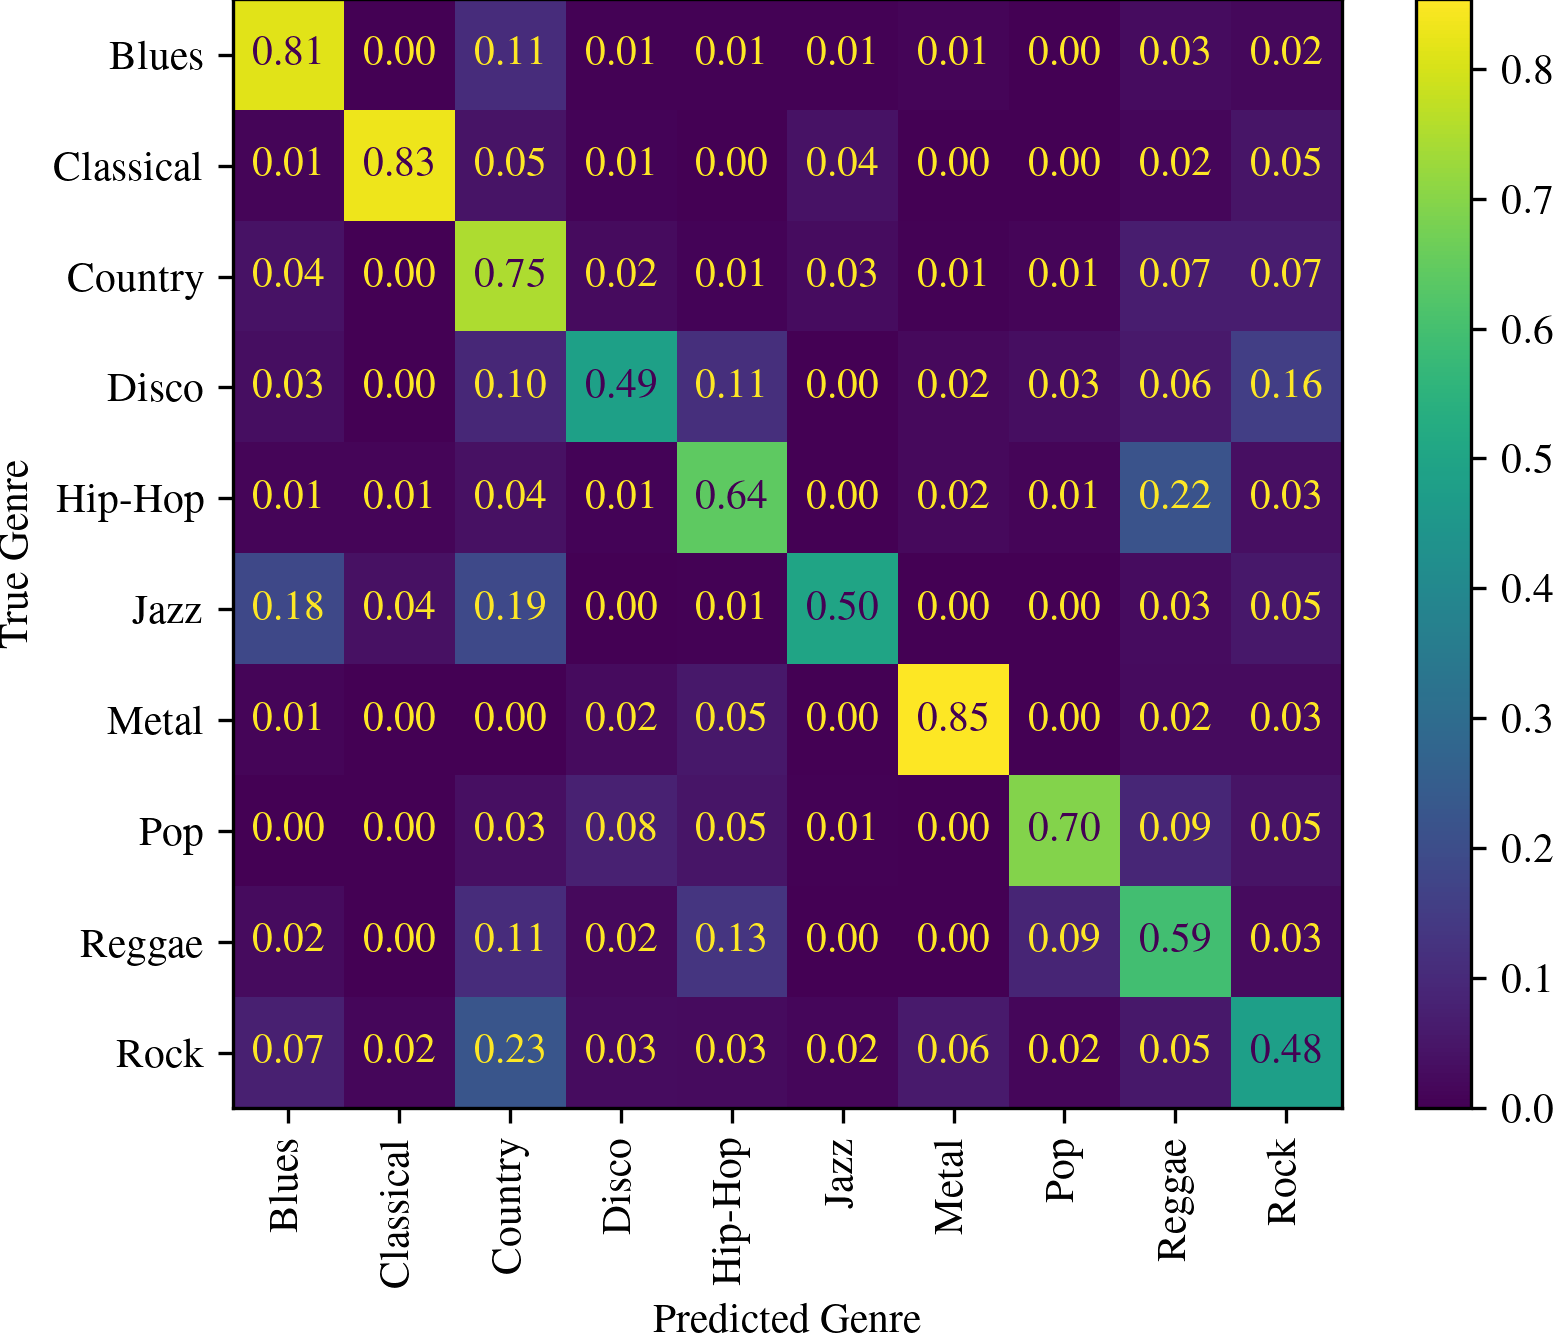
\includegraphics[width=\columnwidth]{cm.png}}
    \caption{Confusion matrix}
    \label{confusion_matrix}
\end{figure}

\section{Training Curves}

Overfitting occurs when a network learns the noise in the data as if it represents the structure of the underlying model.
To detect overfitting, loss and accuracy are important metrics to monitor during training; Figure \ref{accuracy_curves} and Figure \ref{loss_curves} display the accuracy and loss curves for my network, respectively.
For the training set, I logged the loss and accuracy of the batch at the end of each step; for the test set, I logged the loss and accuracy of the entire test set at the end of each epoch.

\begin{figure}[htbp]
    \centerline{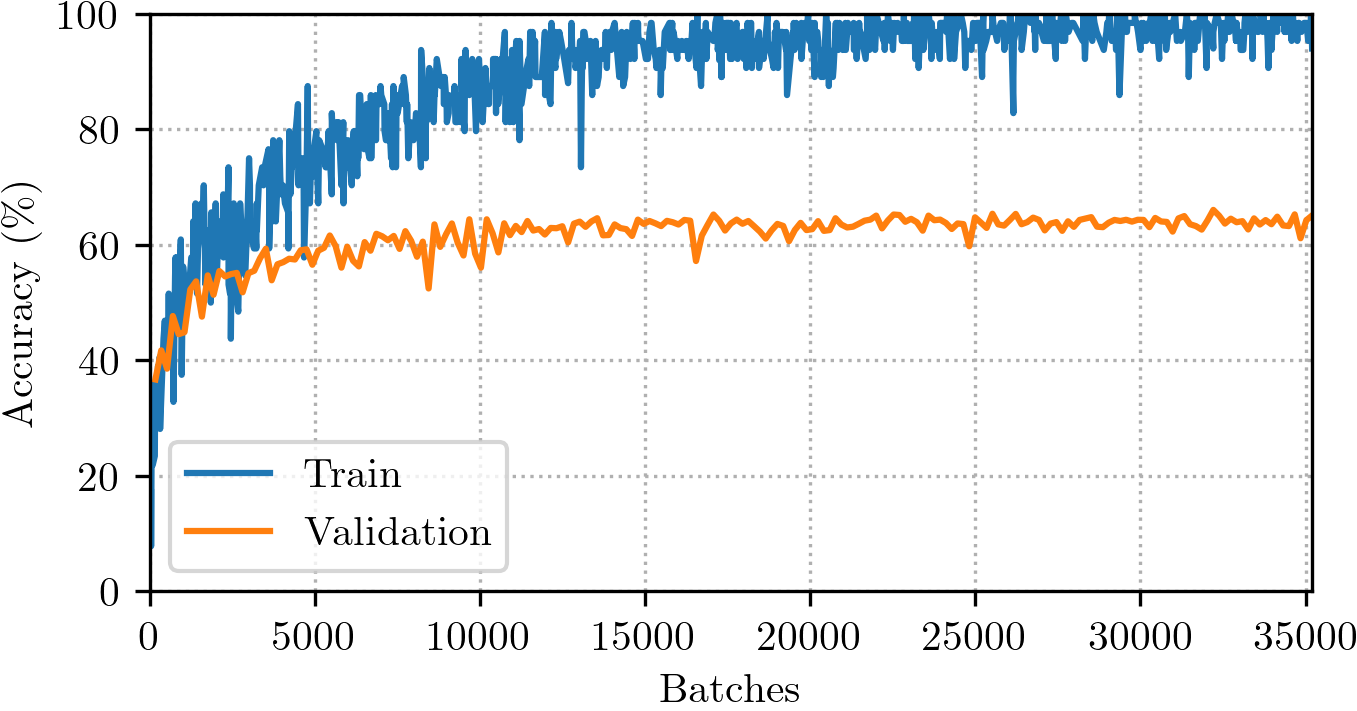
\includegraphics[width=\columnwidth]{accuracy.png}}
    \caption{Accuracy curves}
    \label{accuracy_curves}
\end{figure}

After 200 epochs, there was a discrepency of approximately 35\% in the accuracy of the model on the training and test sets---this strongly indicates that the shallow CNN architecture overfit.
Despite using L1 regularisation and dropout, the model had memorised almost every sample in the training set, and therefore struggled to generalise to unseen data.

\begin{figure}[htbp]
    \centerline{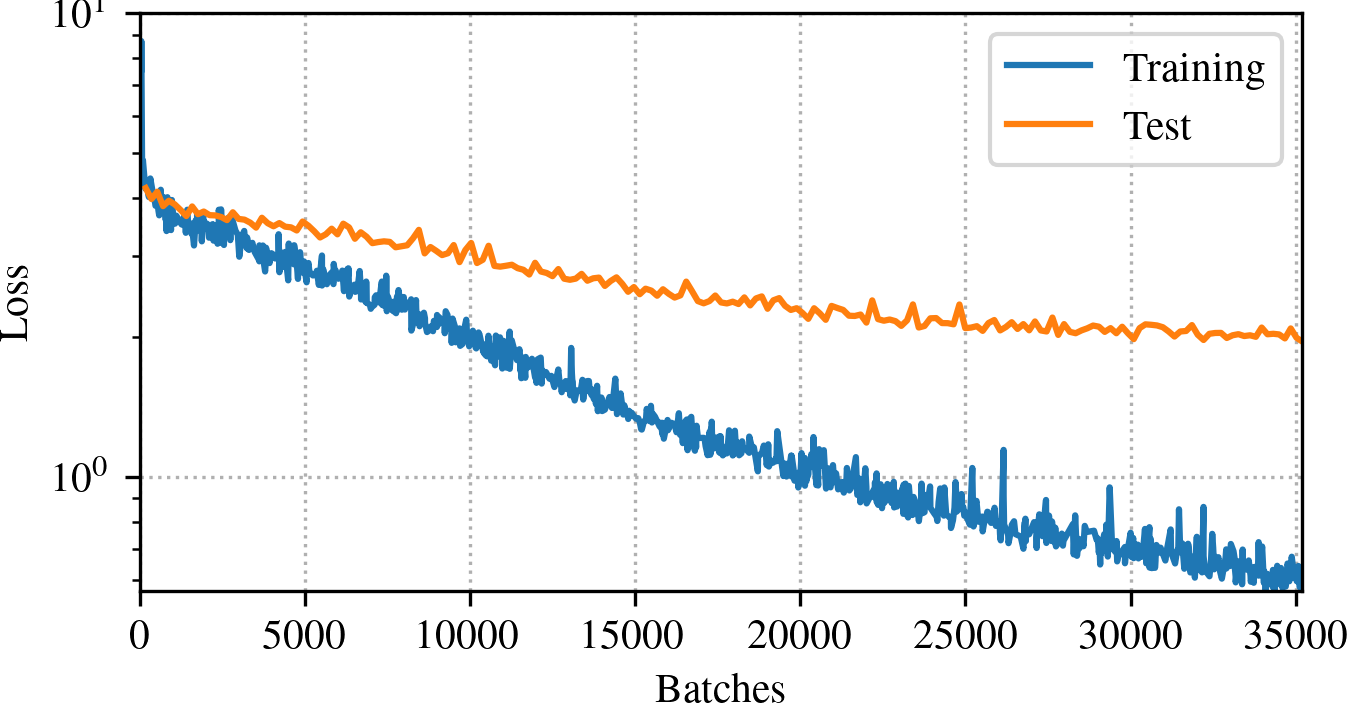
\includegraphics[width=\columnwidth]{loss.png}}
    \caption{Loss curves}
    \label{loss_curves}
\end{figure}

\section{Qualitative Results}

The model achieved a high accuracy on specific genres, but a low accuracy on others, as evidenced by the confusion matrix in Figure \ref{confusion_matrix}.
Notably, it accurately classified samples from the classical and metal genres over 85\% of the time.
While conversely, it only managed to accurately classify approximately 40\% of samples from the rock and reggae genres.

An analysis of the spectrograms from these genres reveals potential reasons for these discrepencies in per-class accuracy.

\section{Improvements}

Thus far, I have computed the `raw' accuracy of my model, by individually predicting the genre for each sample in my dataset.
However, this is not the optimal method, since it ignores all file dependencies; each WAV audio track within the dataset is represented by fifteen 0.93 second samples.
Schindler et al. recognised this, and achieved a substantial improvement in accuracy by introducing two new methods of classification: maximum probability and majority vote---both of which take file dependencies into account.
To classify an inputted audio file by maximum probability, the probabilities output by the final softmax layer for each segment are first summed; then, the predicted class is determined by the largest value amongst the summed probabilities.
To classify an inputted audio file by majority vote, a class is determined for each segment by the largest value output by the final layer; then, a majority vote is conducted over the predicted classes for each of the segments.

Table \ref{improved_results} displays the accuracy achieved using each of the raw, maximum probability and majority vote approaches.
The relative improvement to accuracy provided by maximum probability classification and majority vote classification are consistent with the findings of Schindler et al.

To further improve the performance of my network, I implemented batch normalisation following the two convolutional layers in my network.

\begin{table}[htbp]
    \caption{Improved Accuracy on the Test Set}
    \begin{center}
    \begin{tabular}{l c c c c}
    \toprule
    &&\multicolumn{3}{c}{\textbf{Accuracy}}\\
    \cmidrule(lr){3-5}
    \textbf{Model}&\textbf{Epoch}&\textbf{Raw}&\textbf{Max}&\textbf{Maj}\\
    \midrule
    \multirow{ 2}{*}{My CNN} & 100 & 63.2&&\\
    & 200 & 52.1&&\\
    \midrule
    \multirow{ 2}{*}{My CNN + Batch Norm} & 100 & 66.56&&\\
    & 200 & 67.49&&\\
    \bottomrule
    \end{tabular}
    \label{improved_results}
    \end{center}
\end{table}

\section{Conclusion and Future Work}



\bibliographystyle{IEEEtran}
\bibliography{refs}

\end{document}
